\documentclass[10pt]{article}
\usepackage[margin=0.7in]{geometry}
\usepackage[T1]{fontenc}
\usepackage[utf8]{inputenc}
\usepackage{graphicx}
\usepackage{hyperref}
\usepackage{array}
\usepackage{longtable}
\usepackage{amsmath}
\usepackage{amssymb}
\setlength{\parskip}{0.55em}
\setlength{\parindent}{0pt}
\hypersetup{colorlinks=true,urlcolor=blue,linkcolor=blue}
\title{Native cubic-transfer correctness records}
\author{Research record for PR \#2893}
\date{2026-10-30}
\begin{document}
\maketitle

\textbf{Observation-only report.} This document summarizes already committed
native correctness receipts. It makes no evidence-review decision and does not
claim a practical ECDLP break, a faster general solver, or a performance
advantage.

\section*{Scope and evidence identity}

Reviewed source revision (full hash):
\begin{quote}\small\ttfamily
9c33a7fc7a7af95c6450a90808d2f4e8e74702e9
\end{quote}
The build record is \url{results/native-build-info-20261030.json}. It identifies
the pinned image by digest, C++ and Rust compilers, flags, Singular version,
and a one-CPU, 4-GiB, network-disabled development limit. The matching source
inventory is \url{results/native-sources-20261030.sha256}. These files and the
cited receipts are part of the PR branch.

The source schemas do not define a separate \path{run_id} field. The figures
therefore identify the recorded work by its receipt paths, without inferring
or inventing a run ID:
\begin{itemize}
\item Supplemental panel files: \url{results/panel-development-attempt2/}
\item Panel summary: \url{results/panel-summary-20261030.json}
\item Original p109 IC receipt:
\path{p109-transfer-}\allowbreak\path{ic-final-}\allowbreak\path{20261030.json}
\item Original p109 target-rho receipt:
\path{p109-transfer-}\allowbreak\path{rho-final-}\allowbreak\path{20261030.json}
\item Original p157 IC receipt:
\path{p157-transfer-}\allowbreak\path{ic-final-}\allowbreak\path{20261030.json}
\item Original p157 target-rho receipt:
\path{p157-transfer-}\allowbreak\path{rho-final-}\allowbreak\path{20261030.json}
\end{itemize}

\section*{Inputs and recorded outcomes}

The public input identities are the exact fixtures
\href{../../fixtures/p109.public}{\path{fixtures/p109.public}} and
\href{../../fixtures/p157.public}{\path{fixtures/p157.public}}. They give
\(p=109,\ r=1{,}293{,}169\) and \(p=157,\ r=3{,}868{,}159\), respectively, and
their source elliptic curves over \(\mathbb{F}_{p^3}\). The cubic generators
satisfy \(z^3+z+103=0\) for p109 and \(z^3+z+152=0\) for p157. For p109 the curve is
\(y^2=x^3+(37z^2+105z+29)x+(43z^2+6z+66)\); for p157 it is
\(y^2=x^3+(120z^2+98z+86)x+(101z^2+50z+144)\), with \(z\) as defined by each
fixture. The fixtures contain only public parameters and points. The solver
input omits the known answer scalar.

Two original public instances have final target-solver receipts for both
index-calculus and target-rho arms. Each reports a recovered scalar verified
on its original source curve: p109 records \(k=1729\), and p157 records
\(k=271828\). The additional panel contains sixteen distinct public targets:
eight for each source curve. Its summary records
\path{source_verified=true}, \path{no_synthetic_targets=true}, and
\path{no_source_log_read=true}; all sixteen separately named
\path{*-independent-verification.json} receipts report \path{status=passed}.
Together these are eighteen recorded native correctness instances. They are
not eighteen independent prime-field security instances: there are two toy
source curves and the sixteen extra targets share those sources.

\begin{figure}[ht]
\centering
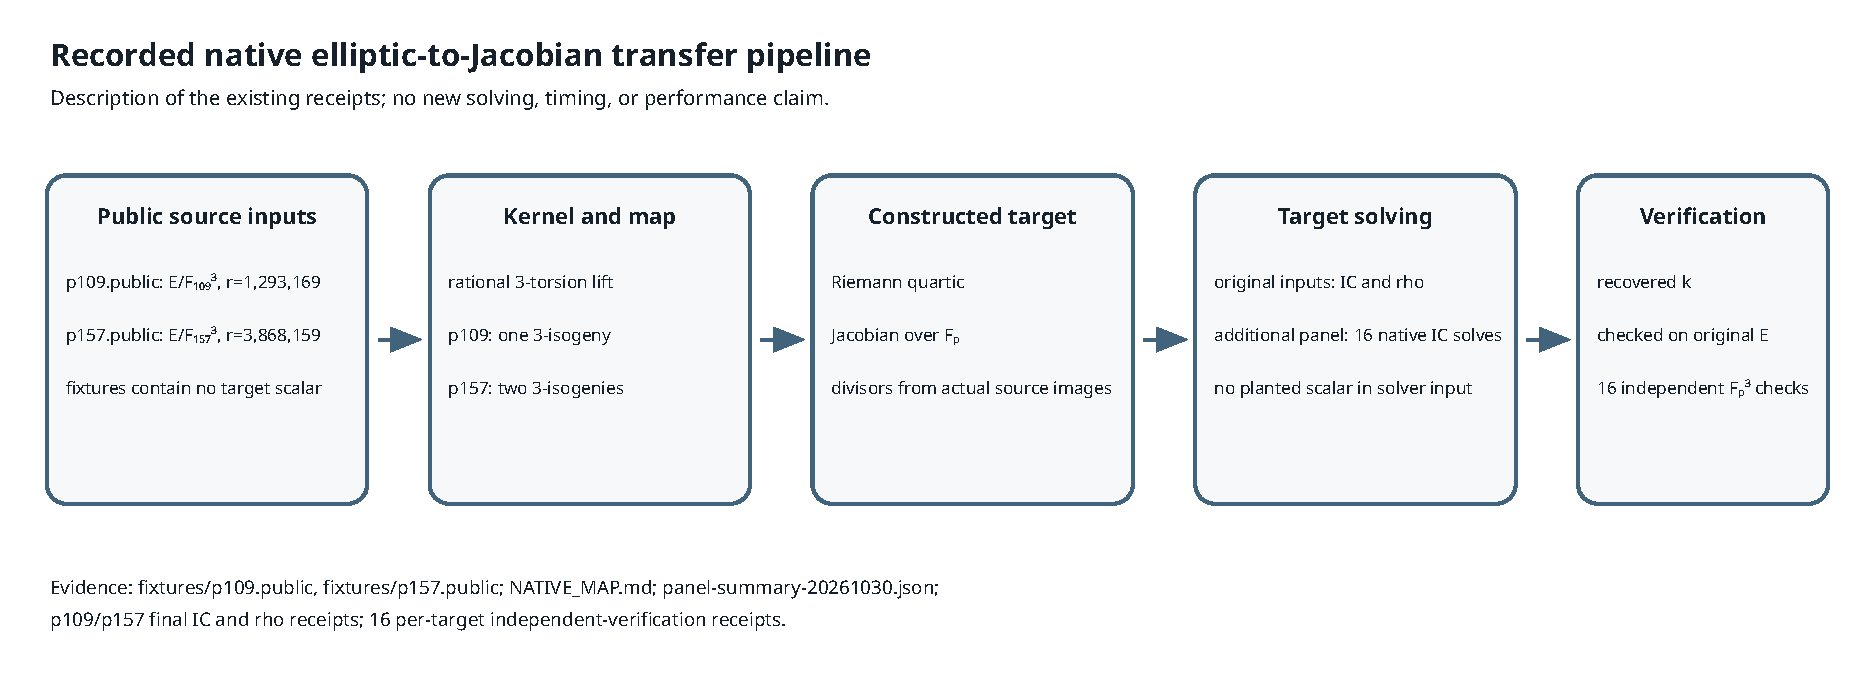
\includegraphics[width=\linewidth]{transfer-pipeline.pdf}
\caption{Stages described by the existing public fixtures, construction
records, final solves, and independent panel verifications. The source
constructs the target quartic from actual source images. The arrows show the
recorded data flow, not a claim that the transfer is universally available.}
\end{figure}

\section*{Recorded panel attempts}

Figure~\ref{fig:attempts} plots the two per-target attempt counts in the
sixteen-case summary: Jacobian base-point attempts and verification split
attempts. The recorded source randomization multiplier is carried in each row
label; it is not an attempt count. No timing, interval, or uncertainty value is
present in the source record. The target labels are joined to the public
known-answer workload list by the recorded source prime and recovered scalar;
the renderer checks that the mapping is one-to-one and covers all sixteen
targets.

\begin{figure}[ht]
\centering
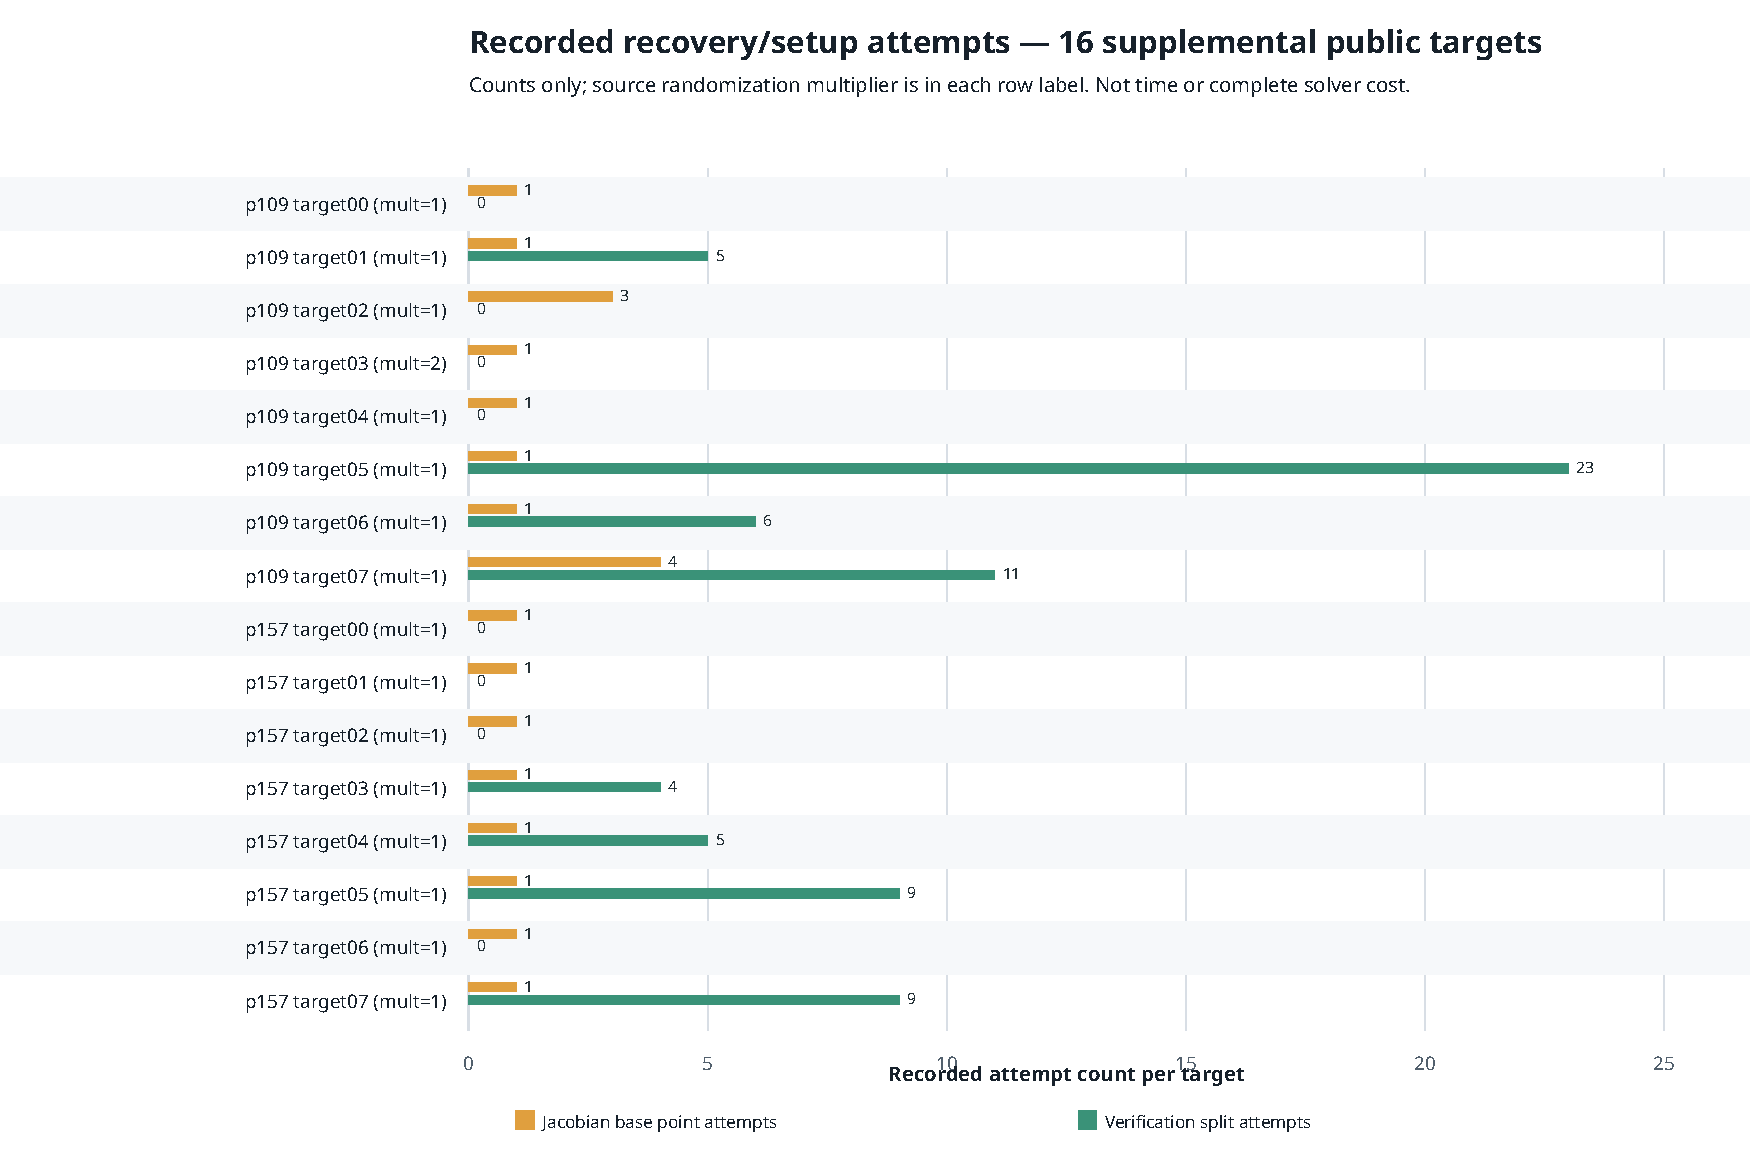
\includegraphics[width=\linewidth]{panel-attempts.pdf}
\caption{Attempt counts for \(n=16\) supplemental public targets. Record
identifier is the source receipt bundle
\protect\url{panel-development-attempt2/}, with summary
\protect\url{panel-summary-20261030.json}; no standalone run-ID field is defined.
Counts are not time or total solver cost, and the panel has no recorded
uncertainty intervals.}
\label{fig:attempts}
\end{figure}

\clearpage
\section*{Original solver counters and limitations}

The four original final receipts declare the same counter scope: the entire
target-solver C ABI call, including checks and verification retries. The table
below copies the recorded counters. It is not a complete end-to-end price:
setup, FLINT and Singular work are not priced, and no wall-time measurement is
admitted. The receipts explicitly have \path{benchmark=false}.

\small
\begin{longtable}{>{\raggedright\arraybackslash}p{0.12\linewidth}
>{\raggedright\arraybackslash}p{0.18\linewidth}
rrrrr}
\hline
Source & Arm & \(I\) & \(LA\) & \(M\) & \(NAT\) & adds \\
\hline
p109 & IC & 612777 & 25227 & 14789496 & 3114 & 732 \\
p109 & target rho & 5221527 & 0 & 125628837 & 2163 & 14702 \\
p157 & IC & 544468 & 33578 & 13222681 & 4137 & 705 \\
p157 & target rho & 2856125 & 0 & 69100315 & 3840 & 8172 \\
\hline
\end{longtable}
\normalsize

The IC and rho records are correctness controls under that declared
target-solver counter scope. These counts do not support a speedup statement.
The build record says full native work is not priced and wall time is not
admitted. It also records that the root release-library validation did not
pass; Rust root sources are unchanged by this implementation. The native
development commands and retry bounds are documented in
\href{../../NATIVE_MAP.md}{\path{NATIVE_MAP.md}}. The original receipts,
failed attempts, and first-panel failed verification remain unchanged.

The only derived operation in the plot is the deterministic label join from a
case's recorded \(p\) and recovered scalar to the corresponding public
known-answer workload. The plotted counts themselves are copied without
aggregation. There are no confidence intervals or sampled estimates to
recompute. Reproduce the visuals without launching any solver:

\begin{verbatim}
python3 make_visuals.py
rsvg-convert -f pdf -o transfer-pipeline.pdf transfer-pipeline.svg
rsvg-convert -f pdf -o panel-attempts.pdf panel-attempts.svg
pdflatex -interaction=nonstopmode -halt-on-error report.tex
\end{verbatim}

\end{document}
